%----------------------------------------------------------------------------------------
%
% LaTeX-template for degree projects at LNU, Department of Computer Science
% Last updated by Johan Hagelbäck, Oct 2015
% Linnaeus University
%
% License: Creative Commons BY
%
%----------------------------------------------------------------------------------------

%----------------------------------------------------------------------------------------
%	Settings and configuration
%----------------------------------------------------------------------------------------

\documentclass[a4paper,12pt]{article}

\usepackage[T1]{fontenc}
\usepackage{times}
\usepackage[english]{babel}
\usepackage[utf8]{inputenc}
\usepackage{wallpaper}
\usepackage[absolute]{textpos}
\usepackage[top=2cm, bottom=2.5cm, left=3cm, right=3cm]{geometry}
\usepackage{appendix}
\usepackage[nottoc]{tocbibind}
\usepackage{enumerate}
\usepackage{array}
\newcolumntype{L}[1]{>{\raggedright\let\newline\\\arraybackslash\hspace{0pt}}m{#1}}


\setcounter{secnumdepth}{3}
\setcounter{tocdepth}{3}

\usepackage{sectsty}
\sectionfont{\fontsize{14}{15}\selectfont}
\subsectionfont{\fontsize{12}{15}\selectfont}
\subsubsectionfont{\fontsize{12}{15}\selectfont}
\usepackage[font=large, labelfont=bf]{caption}

\usepackage{csquotes} % Used to handle citations

\renewcommand{\thetable}{\arabic{section}.\arabic{table}}  
\renewcommand{\thefigure}{\arabic{section}.\arabic{figure}} 

%----------------------------------------------------------------------------------------
%	
%----------------------------------------------------------------------------------------
\newsavebox{\mybox}
\newlength{\mydepth}
\newlength{\myheight}

\newenvironment{sidebar}%
{\begin{lrbox}{\mybox}\begin{minipage}{\textwidth}}%
{\end{minipage}\end{lrbox}%
 \settodepth{\mydepth}{\usebox{\mybox}}%
 \settoheight{\myheight}{\usebox{\mybox}}%
 \addtolength{\myheight}{\mydepth}%
 \noindent\makebox[0pt]{\hspace{-20pt}\rule[-\mydepth]{1pt}{\myheight}}%
 \usebox{\mybox}}

%----------------------------------------------------------------------------------------
%	Title section
%----------------------------------------------------------------------------------------
\newcommand\BackgroundPic{
    \put(-2,-3){
    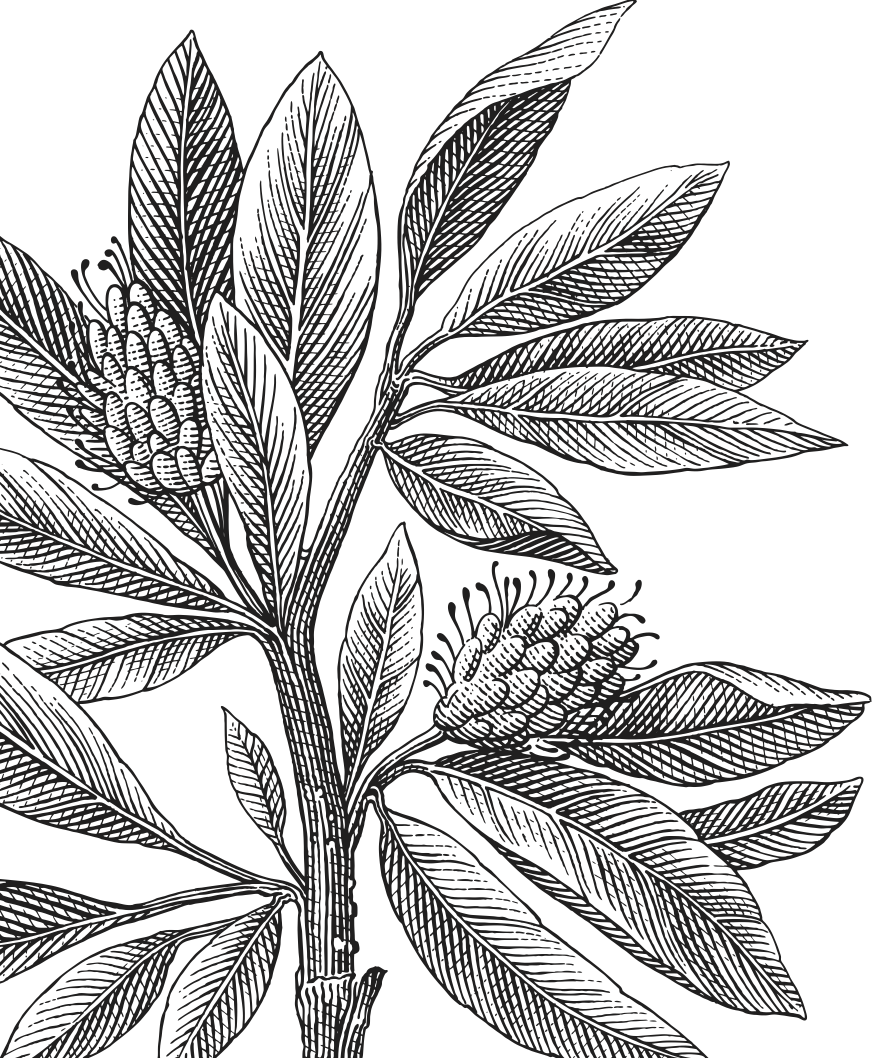
\includegraphics[keepaspectratio,scale=0.3]{img/lnu_etch.png} % Background picture
    }
}
\newcommand\BackgroundPicLogo{
    \put(30,740){
    
\includegraphics[keepaspectratio,scale=0.10]{img/logo.png} % Logo in upper left corner
    }
}

\title{	
\vspace{-8cm}
\begin{sidebar}
    \vspace{10cm}
    \normalfont \normalsize
    \Huge Report \\
    \vspace{-1.3cm}
\end{sidebar}
\vspace{3cm}
\begin{flushleft}
    \huge Project Course In Computer Science\\ 
    \it \LARGE - UML Class Diagram
\end{flushleft}
\null
\vfill
\begin{textblock}{6}(10,13)
\begin{flushright}
\begin{minipage}{\textwidth}
\begin{flushleft} \large
\emph{Author:} Quasim Aljubarah, Michael Johansson, Tadas Lisauskas, Zeyuan Li, Robin Reijo and Robin Stempa\\ % Author
\emph{Supervisor:} Ola Petersson\\ % Supervisor
%\emph{Examiner:} Dr.~Mark \textsc{Brown}\\ % Examiner (course manager)
\emph{Semester:} VT 2016\\ % 
\emph{Subject:} 1DV508\\ % Subject area
\end{flushleft}
\end{minipage}
\end{flushright}
\end{textblock}
}

\date{} 

\begin{document}
\pagenumbering{gobble}
\newgeometry{left=5cm}
\AddToShipoutPicture*{\BackgroundPic}
\AddToShipoutPicture*{\BackgroundPicLogo}
\maketitle
\restoregeometry
\clearpage

\selectlanguage{english}

\tableofcontents

\newpage
\pagenumbering{gobble}
\pagenumbering{arabic}

%----------------------------------------------------------------------------------------
%
%	Here follows the actual text contents of the report.
%
%----------------------------------------------------------------------------------------
\section{Revision History}

\begin{table}[htbp]
	\centering
	\begin{tabular}{|L{4cm}|L{8cm}|L{4cm}|}
		\hline
		\textbf{Change} & \textbf{Description} & \textbf{Name and Date} \\ \hline
		Created Revision history table	&       included a revision history table to the document           &     Michael Johansson, 26/4 -2016               \\ \hline
		Updated Product	&  Updated the class product with more fields and more methods             &        Michael Johansson 26/4 -2016                \\ \hline
		Updated UML diagram	& new classes and updated old ones with more methods and fields		&	Michael Johansson \newline 3/5 -2016  \\ \hline
		Updated UML &	new classes and stuff	& Michael Johansson 10/5 - 2016		\\ \hline
		Updated UML diagram &	Added the latest methods and classes	& Michael Johansson 16/5 - 2016 		\\ \hline
		&		& 		\\ \hline
	\end{tabular}
\end{table}
\newpage
\section{Diagram}

This is our UML class diagram about our web shop. This holds all our classes and a representative image of the database. 

\begin{figure}[htbp]
	\caption{UML class diagram}
	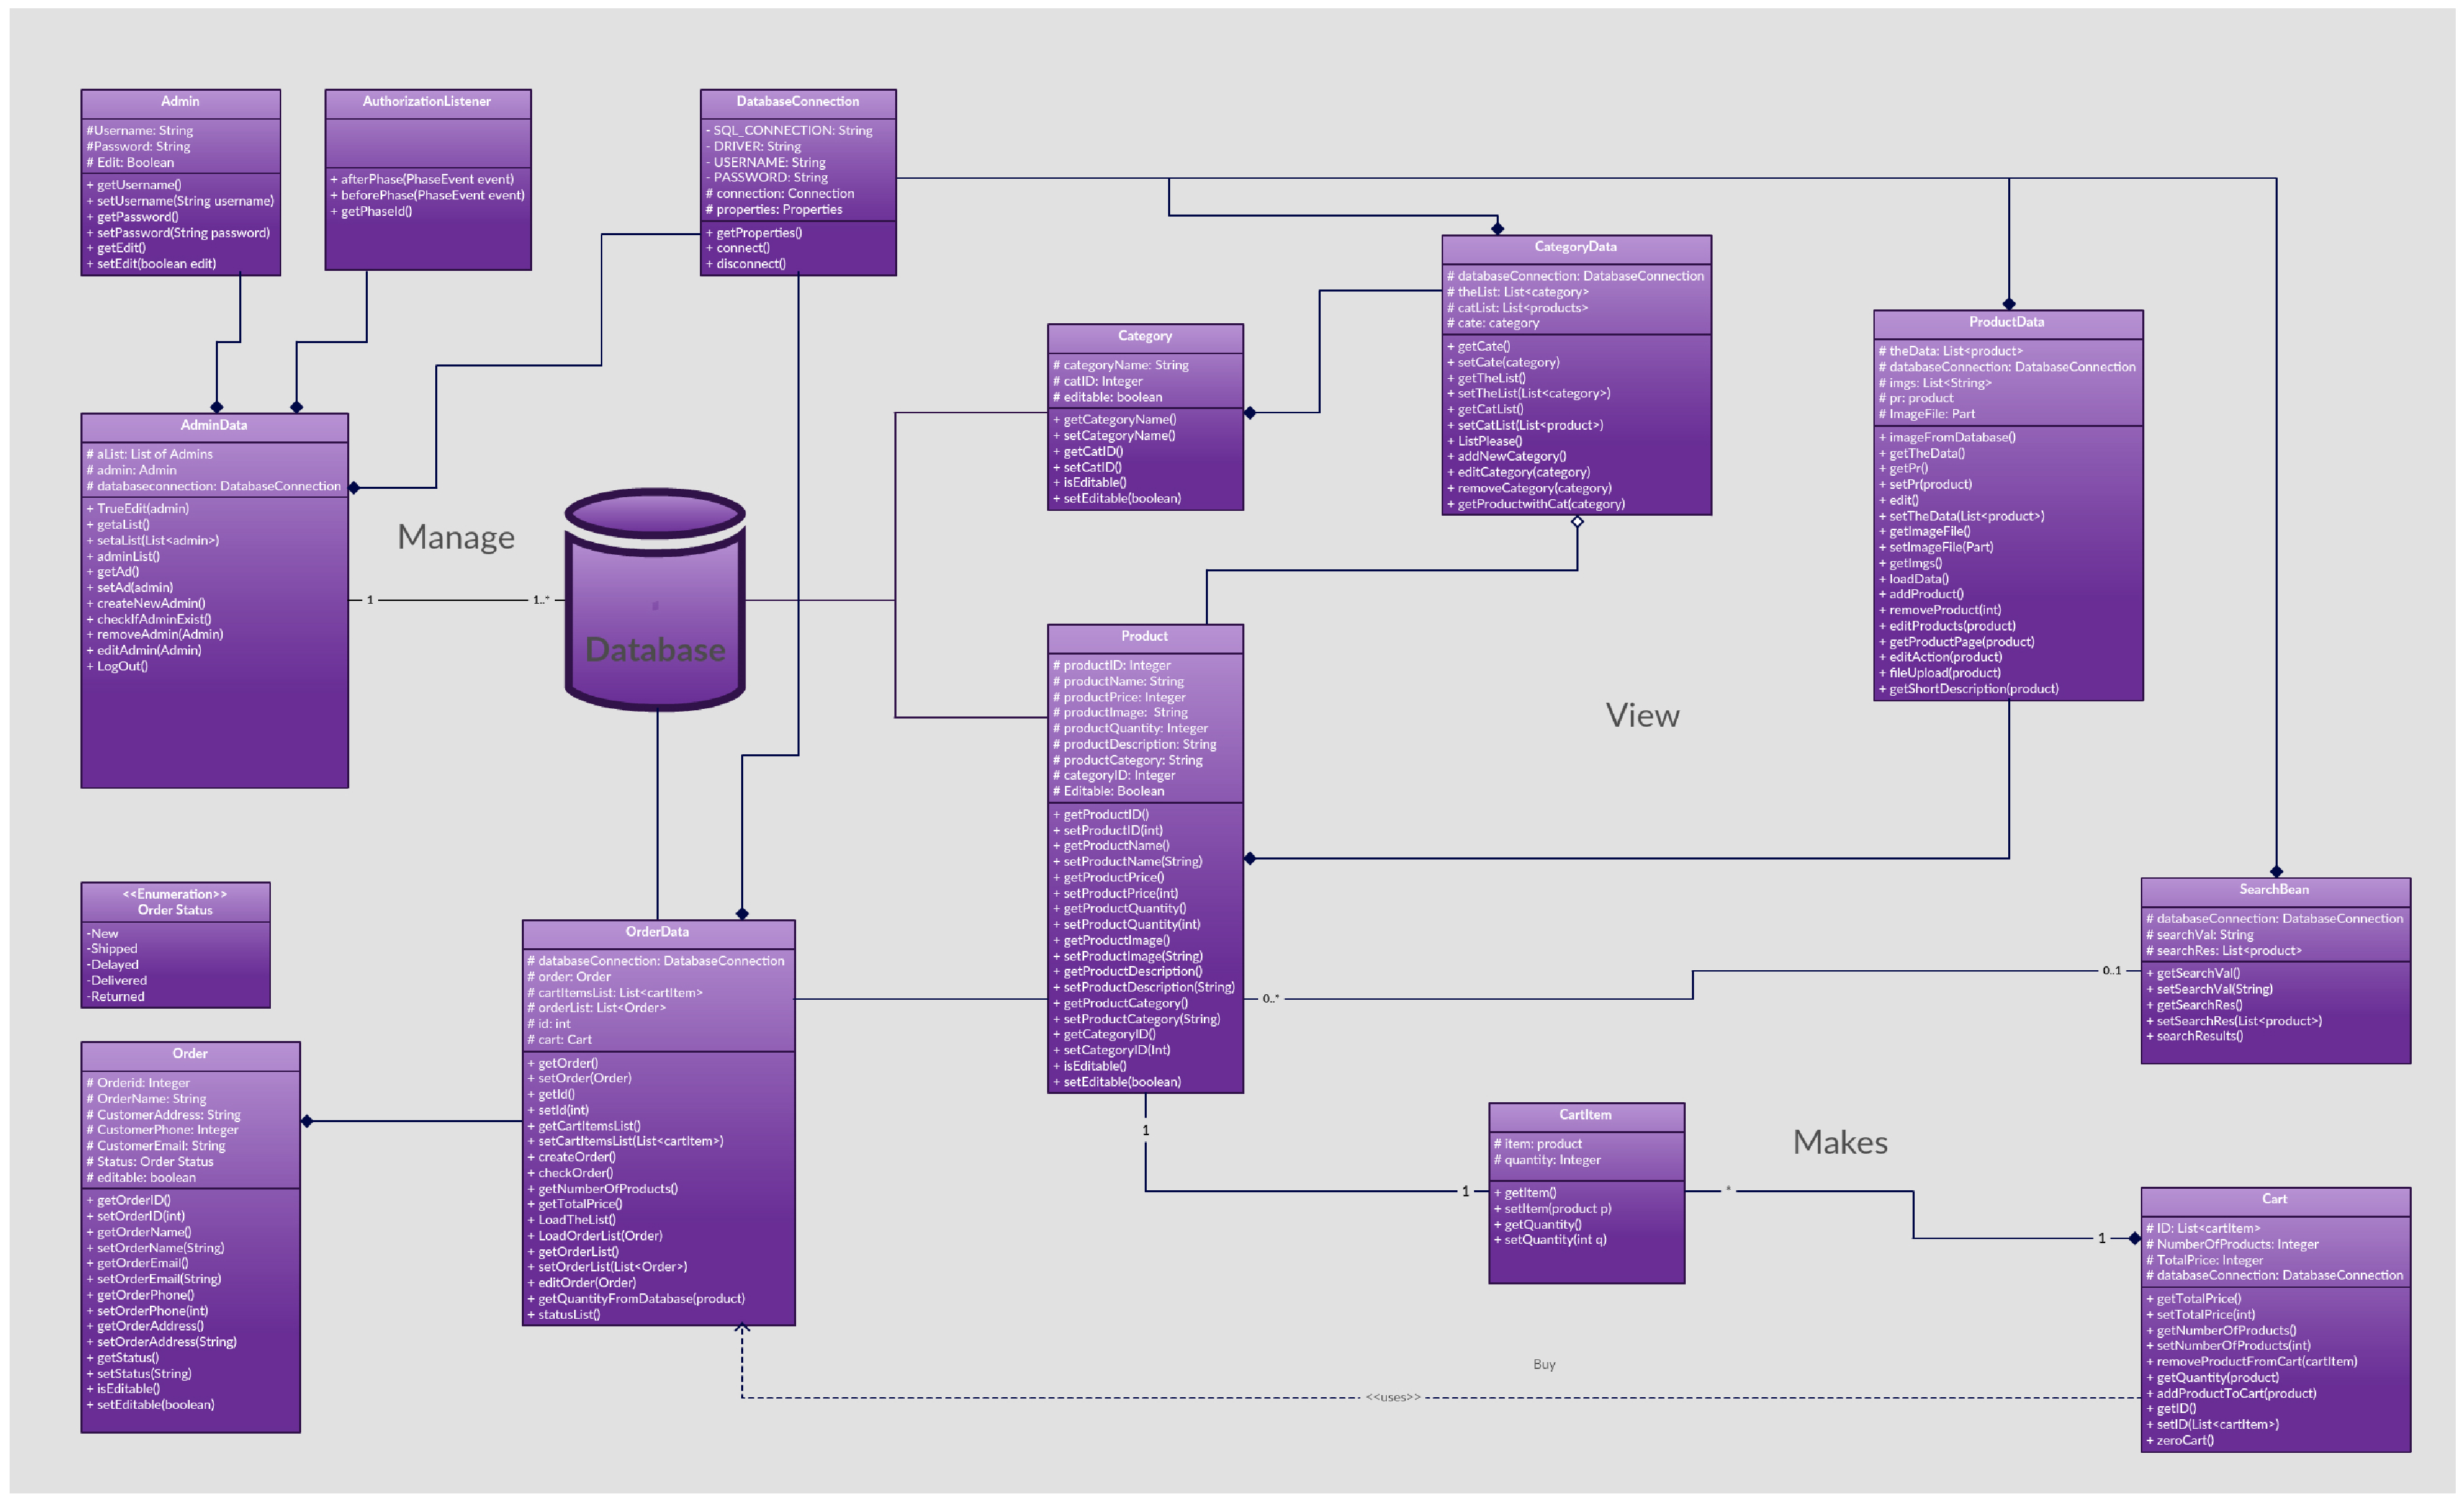
\includegraphics[width=\textwidth, height=\textheight, keepaspectratio]{img/UML.pdf}
\end{figure}

\end{document}
